\section{The Hydrogen Atom}
Den radiale Schrödingerligningen er givet ved\cite{griffiths}
%
\begin{align}
    \frac{-\hbar^{2}}{2m}\diff[2]{u(r)}{r} + \left( - \frac{e^{2}}{4\pi\epsilon_{0}r} + \frac{\hbar^{2}}{2m}\frac{l(l+1)}{r^{2}} \right)u(r) & \nonumber \\
    = Eu(r), & 
    \label{eq:schroedinger3d}
\end{align}

hvor $V_{\text{eff}}$ er en sum af Coulomb potentialet og et led tilhørende et angulært moment.

Fra \cite{griffiths} kendes bohrradien, $a_{0}$ og Rydbergenergien $\mathrm{Ry}$ til følgende værdier;

\begin{align}
    a_{0} = & \frac{\hbar^{2}}{2m}\left( \frac{e^{2}}{4\pi\epsilon_{0}} \right) \\
\mathrm{Ry} = & \frac{m}{2\hbar^{2}}\left( \frac{e^{2}}{4\pi\epsilon_0} \right)^{2}
\label{eq:konstanter}
\end{align} 

Sættes energien til at være et multiplum af Rydbergenergien, $E = -\varepsilon \mathrm{Ry}$, og genkendes det, at $a_{0}^{2}\mathrm{Ry} = \frac{\hbar^{2}}{2m}$, samt at $2a_{0}\mathrm{Ry} = \frac{e^{2}}{4\pi\epsilon_{0}}$, kan \fxnote{reference} skrives
\begin{align}
    k(r) = & \frac{1}{\hbar} \sqrt{2m\left( E - V_{\text{eff}} \right)}\\ 
    = & \sqrt{\frac{1}{a_{0}^{2}\mathrm{\mathrm{Ry}}} \left( E + \frac{e^{2}}{4\pi\epsilon_{0}r} - \frac{\hbar^{2}}{2m}\frac{l(l+1)}{r^{2}} \right)}\\
    = & \sqrt{\frac{1}{a_{0}^{2}\mathrm{Ry}} \left( (-\varepsilon \mathrm{Ry}) + \frac{2a_{0}\mathrm{Ry}}{r} - a_{0}^{2}\mathrm{Ry}\frac{l(l+1)}{r^{2}} \right)}\\
    = & \frac{1}{r} \sqrt{\frac{1}{a_{0}^{2}{Ry}} \left( (-\varepsilon \mathrm{Ry})r^{2} + 2a_{0}\mathrm{Ry} r - a_{0}^{2}\mathrm{Ry} l(l+1) \right)}
\end{align}

Plottes $V_{\text{eff}}$

\begin{figure}[h!]
    \centering
    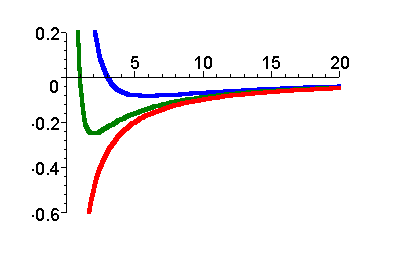
\includegraphics[width=\columnwidth]{hydrogen}
    \caption{Hydrogen}
    \label{fig:hydrogen}
\end{figure}


%
